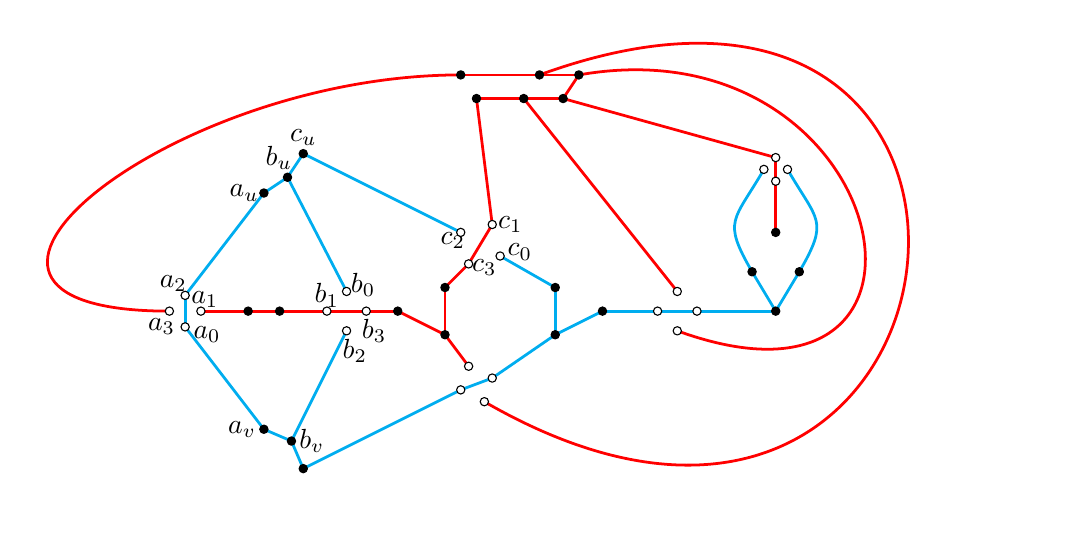
\begin{tikzpicture}[line cap=round,line join=round,x=1cm,y=1cm]
\clip(-3,-.5) rectangle (10,5.6);

\begin{scriptsize}

%
% Node v
%
%\draw (0,0) node {\large $\hat v$};
\draw [line width=1pt,color=cyan] (0,.5) to  (.35,.35); 
\draw [line width=1pt,color=cyan] (.35,.35) to  (.5,0); 

\draw [line width=1pt,color=cyan] (0,.5) to  (-1,1.8); 
\draw [line width=1pt,color=cyan] (.35,.35) to  (1.05,1.75); 
\draw [line width=1pt,color=cyan] (.5,0) to  (2.5,1); 


\draw (0,.5)[anchor=east] node {\normalsize $a_v$};
\draw (.35,.35)[anchor=west] node {\normalsize $b_v$};
%\draw (.5,0)[anchor=north west] node {\normalsize $d_v$};
\draw [fill=black] (0,.5) circle (1.5pt);
\draw [fill=black] (.35,.35) circle (1.5pt);
\draw [fill=black] (.5,0) circle (1.5pt);

\draw [line width=1pt,color=cyan] (-1,1.8) to  (-1,2.2); 
\draw (-.45,1.9) node[anchor=north east] {\normalsize $a_0$};
\draw [fill=white] (-1,1.8) circle (1.5pt);

% ^b
\draw [line width=1pt,color=cyan] (2.5,1) to (2.9,1.15); 
\draw (.9,1.5)[anchor=west] node {\normalsize $b_2$};
\draw [fill=white] (1.05,1.75) circle (1.5pt);
%\draw (2.5,1)[anchor=north] node {\normalsize $d_0$};
\draw [fill=white] (2.5,1) circle (1.5pt);

%
% Node u
%
%\draw (-.2,4.1) node {\large $\hat u$};

\draw [line width=1pt,color=cyan] (0,3.5) to  (.3,3.7); 
\draw [line width=1pt,color=cyan] (.5,4) to  (.3,3.7); 

\draw [line width=1pt,color=cyan] (0,3.5) to  (-1,2.2); 
\draw [line width=1pt,color=cyan] (.3,3.7) to  (1.05,2.25); 
\draw [line width=1pt,color=cyan] (.5,4) to  (2.5,3); 

\draw (-1.15,2.35) node {\normalsize $a_2$};
\draw [fill=white] (-1,2.2) circle (1.5pt);
\draw (1.26,2.33) node {\normalsize $b_0$};
\draw [fill=white] (1.05,2.25) circle (1.5pt);

\draw (2.4,2.9) node {\normalsize $c_2$};
\draw [fill=white] (2.5,3) circle (1.5pt);

% u node path
\draw (-.25,3.5) node {\normalsize $a_u$};
\draw [fill=black] (0,3.5) circle (1.5pt);
\draw (.5,4.2) node {\normalsize $c_u$};
\draw [fill=black] (.5,4) circle (1.5pt);
\draw (.19,3.95) node {\normalsize $b_u$};
\draw [fill=black] (.3,3.7) circle (1.5pt);

%
% Node z
%
%\draw (3.95,2.1) node {\large $\hat z$};
\draw [line width=1pt,color=cyan] (4.3,2) to (6.5,2); 
\draw [line width=1pt,color=cyan] (3.7,2.3) to (3,2.7); 
\draw [line width=1pt,color=cyan] (3.7,1.7) to (2.9,1.15); 

% node path
\draw [line width=1pt,color=cyan] (3.7,2.3) to  (3.7,1.7); 
\draw [line width=1pt,color=cyan] (3.7,1.7) to  (4.3,2); 


%\draw (3.75,1.5) node {\normalsize $d_z$};
\draw [fill=black] (3.7,1.7)circle (1.5pt);
%\draw (3.75,2.47) node {\normalsize $c_z$};
\draw [fill=black] (3.7,2.3)circle (1.5pt);
%\draw (4.3,2.2) node {\normalsize $g_z$};
\draw [fill=black] (4.3,2)circle (1.5pt);

\draw (3.25,2.75) node {\normalsize $c_0$};
\draw [fill=white] (3,2.7)circle (1.5pt);
%\draw (3.05,1.25)[anchor=north] node {\normalsize $d_2$};
\draw [fill=white] (2.9,1.15)circle (1.5pt);

%eF0 -- e3
\draw [line width=1pt,color=red] (3.3,4.7) to  (5.25,2.25);


%
% Node F_0
%
%\draw (3,5.3) node {\large $\hat F_0$};
\draw [line width=1pt,color=red] (2.7,4.7) to  (3.8,4.7); 
\draw [line width=1pt,color=red] (3.8,4.7) to  (4,5); 
\draw [line width=1pt,color=red] (4,5) to  (2.5,5); 

\draw [line width=1pt,color=red] (2.5,5) to[in=180,out=180,looseness=2]  (-1.2,2); 
\draw [line width=1pt,color=red] (4,5) to[in=-20,out=10,looseness=3]  (5.25,1.75); 
\draw [line width=1pt,color=red] (3.5,5) to[in=-30,out=20,looseness=4.5]  (2.8,.85); 

%^c
\draw [line width=1pt,color=red] (2.6,2.6) to  (2.9,3.1);
\draw [line width=1pt,color=red] (2.7,4.7) to  (2.9,3.1);

\draw (-1.3,1.8) node {\normalsize $a_3$};
\draw [fill=white] (-1.2,2)circle (1.5pt);
\draw (3.13,3.1) node {\normalsize $c_1$};
\draw [fill=white] (2.9,3.1)circle (1.5pt);
%\draw (2.9,.6) node {\normalsize $d_1$};
\draw [fill=white] (2.8,.85)circle (1.5pt);


%fF3 -- 
\draw [line width=1pt,color=red] (6.5,3.9) to  (6.5,3);

% ^f
\draw [line width=1pt,color=cyan] (6.8,2.5) to[in=-60,out=60,looseness=1.5] (6.65,3.8);
\draw [line width=1pt,color=cyan] (6.2,2.5) to[in=-120,out=120,looseness=1.5] (6.35,3.8);

\draw [line width=1pt,color=red] (3.8,4.7) to  (6.5,3.95);
%\draw (6.6,4.1) node {\normalsize $f_0$};
\draw [fill=white] (6.5,3.95)circle (1.5pt);
%\draw (6.65,3.55) node {\normalsize $f_2$};
\draw [fill=white] (6.5,3.65)circle (1.5pt);
%\draw (6.85,3.8) node {\normalsize $f_3$};
\draw [fill=white] (6.65,3.8)circle (1.5pt);
%\draw (6.2,3.84) node {\normalsize $f_1$};
\draw [fill=white] (6.35,3.8)circle (1.5pt);


%\draw (2.5,5)[anchor=south] node {\normalsize $a_{F_0}$};
\draw [fill=black] (2.5,5)circle (1.5pt);
%\draw (2.5,4.6) node {\normalsize $c_{F_0}$};
\draw [fill=black] (2.7,4.7)circle (1.5pt);
%\draw (3.5,5)[anchor=south] node {\normalsize $d_{F_0}$};
\draw [fill=black] (3.5,5)circle (1.5pt);
%\draw (4,5)[anchor=north west] node {\normalsize $g_{F_0}$};
\draw [fill=black] (4,5)circle (1.5pt);
%\draw (3.8,4.7)[anchor=north] node {\normalsize $f_{F_0}$};
\draw [fill=black] (3.8,4.7)circle (1.5pt);
%\draw (3.3,4.7)[anchor=north] node {\normalsize $g_{F_0}$};
\draw [fill=black] (3.3,4.7)circle (1.5pt);

%
% Node y
%
%\draw (6.5,2.35) node {\large $\hat y$};

%node path
\draw [line width=1pt,color=cyan] (6.5,2) to  (6.2,2.5); 
\draw [line width=1pt,color=cyan] (6.5,2) to  (6.8,2.5); 


%\draw (6.5,1.8) node {\normalsize $g_y$};
%\draw (6,2.5) node {\normalsize $f_y$};
%\draw (7,2.5) node {\normalsize $f_y$};
\draw [fill=black] (6.5,2)circle (1.5pt);
\draw [fill=black] (6.2,2.5)circle (1.5pt);
\draw [fill=black] (6.8,2.5)circle (1.5pt);


%
% Node F_1
%
%\draw (2.1,2.05) node {\large $\hat F_1$};
%node path
\draw [line width=1pt,color=red] (2.3,2.3) to  (2.3,1.7); 
\draw [line width=1pt,color=red] (1.7,2) to  (2.3,1.7); 

\draw [line width=1pt,color=red] (2.6,2.6) to  (2.3,2.3); 
\draw [line width=1pt,color=red] (2.6,1.3) to  (2.3,1.7); 
\draw [line width=1pt,color=red] (1.7,2) to  (1.3,2); 

% F_1 to F_2
\draw [line width=1pt,color=red] (.8,2) to  (1.3,2); 

%\draw (1.75,2.2) node {\normalsize $b_{F_1}$};
\draw [fill=black] (1.7,2)circle (1.5pt);
%\draw (2.3,1.7)[anchor=north] node {\normalsize $d_{F_1}$};
\draw [fill=black] (2.3,1.7)circle (1.5pt);
%\draw (2.25,2.2)[anchor=west] node {\normalsize $c_{F_1}$};
\draw [fill=black] (2.3,2.3)circle (1.5pt);
\draw (1.4,1.75) node {\normalsize $b_3$};
\draw [fill=white] (1.3,2)circle (1.5pt);

%\draw (2.8,1.4) node {\normalsize $d_3$};
\draw [fill=white] (2.6,1.3)circle (1.5pt);
\draw (2.8,2.55) node {\normalsize $c_3$};
\draw [fill=white] (2.6,2.6)circle (1.5pt);

%
% Node F_2
%
%\draw (0,2.3) node {\large $\hat F_2$};

\draw [line width=1pt,color=red] (-.8,2) to  (-.3,2); 
\draw [line width=1pt,color=red] (.8,2) to  (.3,2);   
\draw [line width=1pt,color=red] (-.3,2) to (.3,2);   

\draw [fill=black] (-.2,2) circle (1.5pt);
%\draw (-.2,1.8) node {\normalsize $a_{F_2}$};
\draw [fill=black] (.2,2) circle (1.5pt);
%\draw (.3,1.8) node {\normalsize $b_{F_2}$};
\draw (-.75,2.15) node {\normalsize $a_1$};
\draw [fill=white] (-.8,2) circle (1.5pt);
\draw (.8,2.2) node {\normalsize $b_1$};
\draw [fill=white] (.8,2) circle (1.5pt);

%
% Node F_3
%
%\draw (6.75,3) node {\large $\hat F_3$};
%\draw (6.3,3) node {\normalsize $f_{F_3}$};
\draw [fill=black] (6.5,3)circle (1.5pt);

%\draw (5,2)[anchor=south] node {\normalsize $g_0$};
\draw [fill=white] (5,2)circle (1.5pt);
%\draw (5.65,2)[anchor=south] node {\normalsize $g_2$};
\draw [fill=white] (5.5,2)circle (1.5pt);
%\draw (5.4,2.25)[anchor=south] node {\normalsize $g_3$};
\draw [fill=white] (5.25,2.25)circle (1.5pt);
%\draw (5.25,1.75)[anchor=north] node {\normalsize $g_1$};
\draw [fill=white] (5.25,1.75)circle (1.5pt);

\end{scriptsize}
\end{tikzpicture}
